  \sectioncounter{2}
  \section{简单的逻辑联结词, 全称量词与存在量词}

  \subsection{知识梳理}
  简单的\myindex{逻辑联结词} (logical connectives) 有: 且 (and, 符号 $\wedge$), 或 (or, 符号 $\vee$) 和非 (not, 符号 $\neg$). 
  只有当命题 $p$, $q$ 都为真时 $p\wedge q$ 才为真, 当 $p$, $q$ 之一为真时 
  $p\vee q$ 就为真, 而 $p$ 与 $\neg p$ 真假恰好相反. 
  有如下真假值表, 表中 T 代表真 (true), F 代表假 (false).
  \begin{table}[htb]
    \small
    \centering
    \caption{命题真假值表}
    \begin{tabular}{ccccc}
      \toprule
      $p$ & $q$ & $p\wedge q$ & $p\vee q$ & $\neg p$\\
      \midrule
      T & T & T & T & F \\
      T & F & F & T & F \\
      F & F & F & F & T \\
      \bottomrule
    \end{tabular}
  \end{table}

  \myindex{全称量词} (universal quantifier) 的符号为 ``$\forall$'' (for all), 表示 ``对所有的'', 
  \myindex{存在量词} (existential quantifier) 的符号为 ``$\exists$'' (exists), 表示 ``存在一个''.
  形如 ``$\forall\, x\in M$, $p(x)$'' 的命题的否定为 
  ``$\exists\, x\in M$, $\neg p(x)$'', 
  而形如 ``$\exists\, x\in M$, $p(x)$'' 的命题的否定为 
  ``$\forall\, x\in M$, $\neg p(x)$''. 例如 ``$\forall\, x>1$, $x^2>1$'' 
  的否定为 ``$\exists\, x>1$, $x^2\leqslant 1$''. 注意命题的否定和否命题不一样, 
  两者是分别对不同形式的命题进行变化.
  
  由于命题和其否定真假相反, 有时判断命题的真假可以转化为判断其否定的真假. 判断含全称量词或存在量词的命题的真假时, 前者需要检验所考虑范围中的所有变量, 后者只需尝试寻找一个合题意的变量.

  \lianxi
  \begin{exercise}
    若命题 $p\colon \exists\, x\in \mathbb{R}$, $x^2 +x+1=0$, 
    则 $\neg p$ 为\,?
  \end{exercise}

  \beginsolution
    $\neg p\colon \forall\, x\in \mathbb{R}$, $x^2 +x+1\neq 0$.
  \endsolution
  
  \begin{exercise}
    ``$\forall\, x\in \mathbb{R}$, $2x^2-3x+4>0$'' 的否定为\,?
  \end{exercise}

  \beginsolution
    $\exists\, x\in \mathbb{R}$, $2x^2-3x+4\leqslant 0$.
  \endsolution
  
  \begin{exercise}
    命题 ``存在 $a\in \mathbb{R}$, 
    使得函数 $f(x)=x^2 +\dfrac{a}{x}$ ($a\in \mathbb{R}$) 是偶函数'' 
    是$\underline{\qquad}$命题. (填 ``真'' 或 ``假''.)
  \end{exercise}

  \beginsolution
    $f(x)$ 为偶函数 $\Leftrightarrow f(x)=f(-x)\Leftrightarrow a=0$, 填 ``真''.
  \endsolution
  
  \begin{exercise}
    已知命题 $p\colon \forall\, x\in \mathbb{R}$, $\sin x+\cos x>m$ 是真命题,
    那么实数 $m$ 的取值范围是\,?
  \end{exercise}

  \beginsolution
    $\sin x+\cos x= \sqrt2\sin\Big(x+\frac\pi4\Big)\in [-\sqrt2,\sqrt2]$, 
    \mymarginpar{类似地, \\
      (1) $\forall\, x\in D$, $f(x)\leqslant m\Leftrightarrow f_{\max}\leqslant m$;\\
      (2) $\exists\, x_0\in D$, $f(x_0)<m\Leftrightarrow f_{\min}<m$;\\
      (3) $\exists\, x_0\in D$, $f(x)\geqslant m\Leftrightarrow f_{\max}\geqslant m$,\\
      即存在性问题或恒成立问题可化为值域问题. 思考下面两个问题应如何转化:\\
      (1) $\exists\, x_0\in D$, $f(x_0)=m$;\\
      (2) $\exists\, x\in X$, $\forall\, y\in Y$, $f(x)<g(y)$.}
    所以 $m<-\sqrt2$, 即 $m\in(-\infty,-\sqrt2)$.
    
    一般化: $\forall\, x\in D$, $f(x)>m\Leftrightarrow f_{\min}>m$.
  \endsolution
  
  \subsection{要点导学\quad 各个击破}
  \subsubsection{含量词的命题的否定}
  \begin{example}
    命题 ``$\forall\, x\in \mathbb{R}$, $x^2-2x+2>0$'' 的否定是\,?
  \end{example}

  \beginsolution
    $\exists\, x\in \mathbb{R}$, $x^2-2x+2\leqslant 0$. (原命题为真, 其否定为假.)
  \endsolution
  
  \lianxi
  \begin{exercise}[s]
    (1) 命题 ``存在一个无理数, 它的平方是有理数'' 的否定是\,?
    
    (2) 若命题 $p\colon \forall\, x\in\mathbb{R}$, $\sin x\leqslant1$, 
    则 $\neg p$ 是\,?
  \end{exercise}

  \beginsolution
    (1) 对所有的无理数, 它们的平方都是无理数. (原命题为真, 其否定为假.)
    
    (2) $\neg p\colon \exists\, x\in\mathbb{R}$, $\sin x>1$. (原命题为真, 其否定为假.)
  \endsolution
  
  \subsubsection{含量词命题的真假判定}
  \begin{example}
    下列四个命题中正确的命题是\,? (填序号)
    
    (1) $\exists\, x\in (0,+\infty)$, 
      $\Big(\dfrac12\Big)^x> \Big(\dfrac13\Big)^x$;
      
    (2) $\exists\, x\in (0,+\infty)$, $\log_2 x<\log_3 x$;
    
    (3) $\forall\, x\in (0,+\infty)$, $\Big(\dfrac12\Big)^x> \log_{\frac12} x$;
    
    (4) $\forall\, x\in \Big(0,\dfrac13\Big)$, 
      $\Big(\dfrac12\Big)^x< \log_{\frac13} x$.
  \end{example}

  \beginsolution
    方法一: 作图知, (1), (2), (4) 为真, (3) 为假. 作图时, 除了要考虑各函数图象的增减性, 还需注意它们的相对位置. 各题对应图如下:\\
    \rlap{\small
    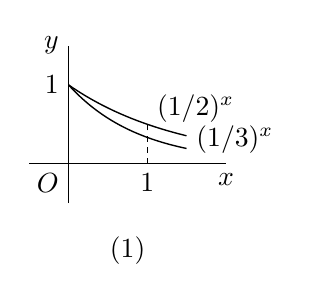
\begin{tikzpicture}[scale=1]
      \draw[\myaxisarrow] (-0.5,0) -- (2,0) node[below] {$x$};
      \draw[\myaxisarrow] (0,-0.5) -- (0,1.5) node[left] {$y$};
      \draw[line width=0.5pt,dash pattern= on 2pt off 2pt] 
        (1,0)--(1,0.5);
      \draw[line width=0.5pt,smooth,samples=100,domain=0:1.5] 
        plot(\x,{0.5^(\x)});
      \draw[line width=0.5pt,smooth,samples=100,domain=0:1.5] 
        plot(\x,{(1/3)^(\x)});
      \draw (0,0) node[anchor= north east] {$O$};
      \draw (1,0) node[below] {$1$} (0,1) node[left] {$1$}
        (1,0.7) node[right] {$(1/2)^x$}
        (1.5,0.3) node[right] {$(1/3)^x$}
        (0.75,-1.1) node {(1)};      
    \end{tikzpicture}\qquad
    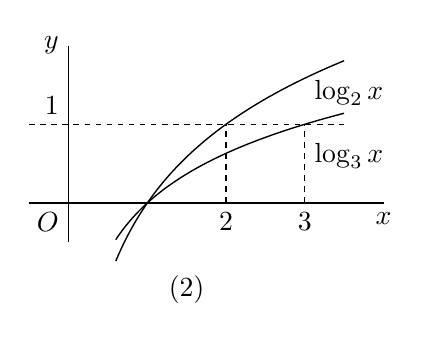
\begin{tikzpicture}[scale=1]
      \draw[\myaxisarrow] (-0.5,0) -- (4,0) node[below] {$x$};
      \draw[\myaxisarrow] (0,-0.5) -- (0,2) node[left] {$y$};
      \draw[line width=0.5pt,dash pattern= on 2pt off 2pt] 
        (-0.5,1)--(3.5,1) (2,0)--(2,1) (3,0)--(3,1);
      \draw[line width=0.5pt,smooth,samples=100,domain=0.6:3.5] 
        plot(\x,{ln(\x)/ln(2)});
      \draw[line width=0.5pt,smooth,samples=100,domain=0.6:3.5] 
        plot(\x,{ln(\x)/ln(3)});
      \draw (0,0) node[anchor= north east] {$O$};
      \draw (0,1) node[anchor= south east] {$1$} (2,0) node[below] {$2$} 
        (3,0) node[below] {$3$} 
        (3,1.4) node[right] {$\log_2 x$}
        (3,0.6) node[right] {$\log_3 x$}
        (1.5,-1.1) node {(2)};      
    \end{tikzpicture}\qquad
    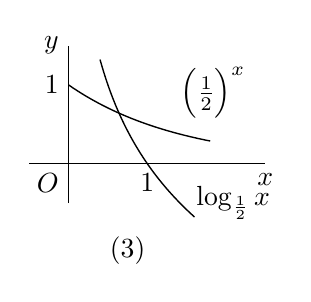
\begin{tikzpicture}[scale=1]
      \draw[\myaxisarrow] (-0.5,0) -- (2.5,0) node[below] {$x$};
      \draw[\myaxisarrow] (0,-0.5) -- (0,1.5) node[left] {$y$};
      \draw[line width=0.5pt,smooth,samples=100,domain=0:1.8] 
        plot(\x,{0.5^(\x)});
      \draw[line width=0.5pt,smooth,samples=100,domain=0.4:1.6] 
        plot(\x,{ln(\x)/ln(0.5)});
      \draw (0,0) node[anchor= north east] {$O$};
      \draw (1,0) node[below] {$1$} (0,1) node[left] {$1$}
        (1.3,0.9) node[right] {$\Big(\frac12\Big)^x$}
        (1.5,-0.5) node[right] {$\log_{\frac12} x$}
        (0.75,-1.1) node {(3)};      
    \end{tikzpicture}\qquad
    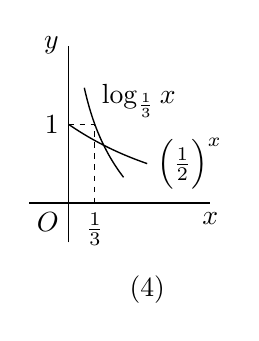
\begin{tikzpicture}[scale=1]
      \draw[\myaxisarrow] (-0.5,0) -- (1.8,0) node[below] {$x$};
      \draw[\myaxisarrow] (0,-0.5) -- (0,2) node[left] {$y$};
      \draw[line width=0.5pt,dash pattern= on 2pt off 2pt] 
        (0,1)--(1/3,1)--(1/3,0);
      \draw[line width=0.5pt,smooth,samples=100,domain=0:1] 
        plot(\x,{0.5^(\x)});
      \draw[line width=0.5pt,smooth,samples=100,domain=0.2:0.7] 
        plot(\x,{ln(\x)/ln(0.333333)});
      \draw (0,0) node[anchor= north east] {$O$};
      \draw (1/3,0) node[below] {$\frac13$} (0,1) node[left] {$1$}
        (1,0.5) node[right] {$\Big(\frac12\Big)^x$}
        (0.3,1.3) node[right] {$\log_{\frac13} x$}
        (1,-1.1) node {(4)};      
    \end{tikzpicture}}
    
    方法二: 找特例或推导, 如 (1) 中取 $x=1$, (2) 和 (3) 中取 $x=\frac12$, (4) 中  $\Big(\dfrac12\Big)^x<1< \log_{\frac13} x$ (找中间值).
    \mymarginpar{比大小时, 常用的中间值是 $-1$, $0$ 和 $1$.}
  \endsolution
  
  \subsubsection{结合命题的真假求参数的值或范围}
  \begin{example}
    已知命题 $p$: $\forall\,x\in [2,4]$, $\log_2 x-a\geqslant 0$, 
    命题 $q$: $\exists\,x\in \mathbb{R}$, $x^2 +2ax+2-a=0$. 
    若 ``$p$ 且 $q$'' 是真命题, 则实数 $a$ 的取值范围是\,?
  \end{example}

  \beginsolution
    $p$, $q$ 均为真, 则 $(\log_2 x)_{\min} \geqslant a$ 且 $(2a)^2-4(2-a)\geqslant 0$, 解得 $a\in(-\infty,-2]\cup\{1\}$.
  \endsolution
  
  \lianxi
  \begin{exercise}[s]
    若命题 ``$\exists\,x\in \mathbb{R}$, $x^2 +2x+m\leqslant 0$'' 是假命题, 
    则 $m$ 的取值范围是\,?
  \end{exercise}

  \beginsolution
    命题 ``$\forall\,x\in \mathbb{R}$, $x^2 +2x+m> 0$'' 是真命题, 则 $\Delta=2^2-4m<0$, $m\in(1,+\infty)$.
  \endsolution
  
  \subsubsection{课堂评价}
  \begin{exercise}
    已知命题 $p\colon \forall\, x\in \mathbb{R}$, $x>\sin x$, 
    那么命题 $p$ 的否定是\,?
  \end{exercise}

  \beginsolution
    $\neg p\colon \exists\, x\in \mathbb{R}$, $x\leqslant\sin x$. (原命题为假, 其否定为真.)
  \endsolution
  
  \begin{exercise}
    已知命题 $p\colon \exists\, x\in [1,2]$, $x^2 +1\geqslant a$, 
    命题 $q\colon \exists\, x\in \mathbb{R}$, $x^2 +ax+1=0$. 
    若命题 $p\vee q$ 为真命题, 则实数 $a$ 的取值范围是\,?
  \end{exercise}

  \beginsolution
    $p$ 或 $q$ 为真, 则 $(x^2+1)_{\max}\geqslant a$ 或 $\Delta= a^2-4\cdot 1\geqslant 0$, 解得 $a\in(-\infty,-2]\cup [2,5]$.
  \endsolution
  
  \subsection{课后练习}
  \begin{exercise}
    下列命题中的假命题是\,? (填序号)
    
    (1) $\forall\, x\in \mathbb{R}$, $2^{x-1}>0$;\qquad
    (2) $\forall\, x\in \mathbb{N}^*$, $(x-1)^2>0$;
    
    (3) $\exists\, x\in \mathbb{R}$, $\lg x<1$;\qquad 
    (4) $\exists\, x\in \mathbb{R}$, $\tan x=2$.
  \end{exercise}

  \beginsolution
    (1) 真; (2) 取 $x=1$ 知, 假; (3) 取 $x=1$ 知, 真; (4) 由正切线知, 真.
  \endsolution
  
  \begin{exercise}
    已知命题 $p\colon \forall\, x\in \mathbb{R}$, $2^x<3^x$,
    命题 $q\colon \exists\, x\in \mathbb{R}$, $x^3 =1-x^2$,
    那么下列命题中为真命题的是\,?
    
    (1) $p\wedge q$;\qquad (2) $\neg p\wedge q$;\qquad
    (3) $p\vee \neg q$.
  \end{exercise}

  \beginsolution
    作图知, $p$ 假 $q$ 真, 故 (1), (3) 真.
  \endsolution
  
  \begin{exercise}
    若命题 ``$\exists\, x_0\in \mathbb{R}$, $x_0^2+ 2ax_0+2-a=0$'' 是真命题,
    则实数 $a$ 的取值范围是\,?
  \end{exercise}

  \beginsolution
    $\Delta= (2a)^2-4(2-a)\geqslant 0$, 则 $a\in(-\infty,-2]\cup[1,+\infty)$.
  \endsolution
  
  \begin{exercise}
    在一次跳伞训练中, 甲、乙两位学员各跳一次. 设命题 $p$ 是 ``甲降落在指定范围内'',
    命题 $q$ 是 ``乙降落在指定范围内'', 则命题 ``至少有一位学员没有降落在指定范围内'' 
    应表示为\,? (填序号)
    
    (1) $\neg p\vee \neg q$;\qquad (2) $p\vee \neg q$;\qquad
    (3) $\neg p\wedge \neg q$;\qquad (4) $p\vee q$.
  \end{exercise}

  \beginsolution
    甲没有降落在指定范围内或乙没有降落在指定范围内, 选 (1).
  \endsolution
  
  \begin{exercise}
    命题 $p$: 函数 $f(x)=x^2 -3ax+4$ 在 $[1,+\infty)$ 上单调递增,
    命题 $q$: 指数函数 $g(x)=(2a-1)^x$ 为减函数. 若 $p\wedge q$ 为假命题,
    求实数 $a$ 的取值范围.
  \end{exercise}

  \beginsolution
    $p$ 或 $q$ 为假, 则 $-\frac{-3a}2\geqslant 1$ 或 $2a-1>1$, 解得 $a\in(1,+\infty)$.
  \endsolution
  
  \begin{exercise}
    命题 $p$: 函数 $f(x)=\log_a x$ 在 $(0,+\infty)$ 上单调递增, 
    命题 $q$: 关于 $x$ 的方程 $x^2-2ax+4=0$ 有实数根.
    若 $p\vee q$ 为真命题, 求实数 $a$ 的取值范围.
  \end{exercise}

  \beginsolution
    $p$ 或 $q$ 为真, 则 $a>1$ 或 $(2a)^2-4\cdot 4\geqslant 0$, 解得 $a\in(-\infty,-2]\cup(1,+\infty)$.
  \endsolution
  
%%%%%%%%%%%%%%%%%%%%%%%%%